\label{chap.4}

\section{Overview}
The four phases of the proposed pipeline (Table~\ref{tab:pipeline}) can only be evaluated collectively, if the forecast, allocation and the resulting service quality are known for the same cell within the same interval. This chapter outlines this: the formulation of the slicing task, unified environment for evaluation of forecast and allocations in the testbed, calibration process for the testbed's quality-of-service (QoS) model, and reference policies used to compare learned controllers.

A dataset that links these phases would have to hold, in one record, the network topology, the traffic of each cell over time, the demand of each slice, QoS measures, the SLA outcome, and the allocation action with its reward. We reviewed the datasets we hold and searched for others, and none has all of these. The closest are the B5G slicing dataset, which covers only the transport network and has no allocation actions, and published O-RAN slicing traces, which come from single-cell testbeds and whose release we could not verify. We therefore built the unified environment synthetically, based on real data wherever real data exist.

\section{System Architecture}
The architecture of the proposed system consists of eight stages, as shown in Figure~\ref{fig:arch}. Network data are gathered from multiple sources (stage 1). Self-supervised learning learns representations from unlabelled network data (stage 2), while the temporal graph neural network makes predictions for future traffic and network states using temporal graphs (stage 3). Multiple MARL agents make joint decisions (stage 4). These decisions are executed in the Digital Twin, which is a virtual copy of the network (stage 5), and resources are assigned to the network slices according to the predictions (stage 6). The network state in the Digital Twin is updated (stage 7), and its performance is evaluated to calculate the reward to improve the policies of the agents (stage 8). Stages 5 to 8 are implemented in the unified environment presented in Section~\ref{sec:env}.
 
\begin{figure}[h]
\centering
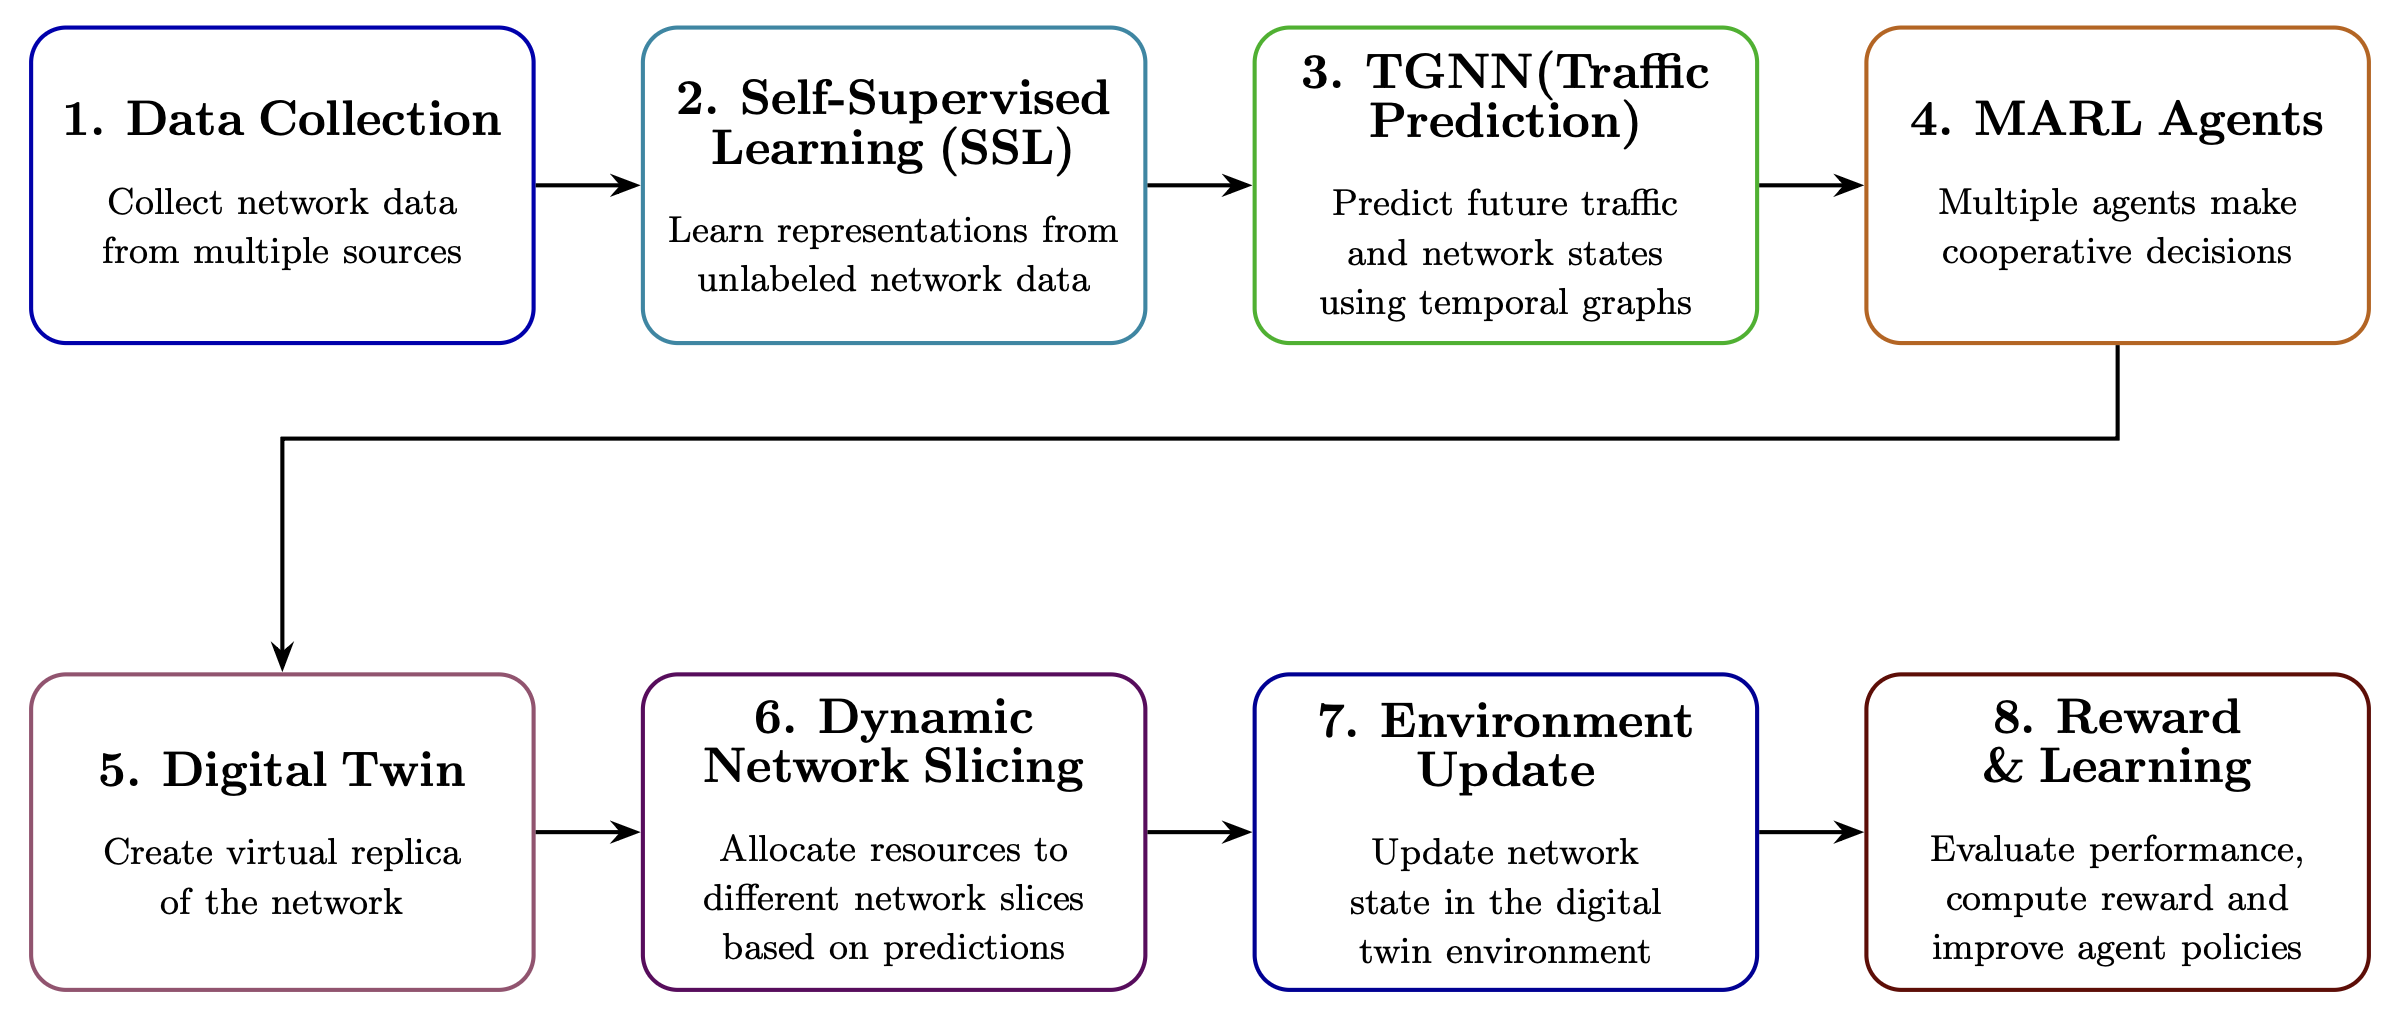
\includegraphics[width=\textwidth]{arch_diag.png}
\caption{Architecture of the proposed system}
\label{fig:arch}
\end{figure}

 
\section{Problem Formulation}
Each cell is controlled by one agent. The agent splits the capacity of its cell into four portions for each of eMBB, URLLC, mMTC and idle and applies the selected portions to the next interval, and so on. Each agent in MARL takes an action only based on 17 local features for their own cell. The load of neighbouring cells diminishes the capacity of a cell (Section~\ref{sec:env}), which means that the decisions of the agents are coupled, and the task is a decentralised multi-agent control problem.

The reward of the agent of cell $i$ in interval $t$ is
\begin{equation}
R_t^{i} = 0.7\,S_t^{i} + 0.3\,F_t^{i} - 0.1\,H_t^{i},
\label{eq:reward}
\end{equation}
where $S_t^{i}$ is a weighted SLA score, $F_t^{i}$ is a fraction of demand that is satisfied and $H_t^{i}$ is a reconfiguration churn. The weights are design choices. The reward therefore favours meeting the SLA targets of the three slices first, then serving demand, and penalises changes of the allocation. During training, each agent's reward is mixed with those of its neighbours (the team reward).

\section{The Unified Slicing Environment}
\label{sec:env}
The environment brings together real traffic on a real spatial layout, per-slice demand, an allocation action, and the resulting QoS, SLA outcome and reward for each cell and each 10-minute interval. It is implemented in the \texttt{src/unified} folder of the project repository. Table~\ref{tab:env} shows which components are real, which are calibrated and which are modelling assumptions.



\begin{table}[h]
\centering
\caption{Components of the unified environment}
\label{tab:env}
\small
\begin{tabular}{|p{3.4cm}|p{2.2cm}|p{9.6cm}|}
\hline
\textbf{Component} & \textbf{Status} & \textbf{Source or rule} \\ \hline
Traffic per cell and interval & Real & Telecom Italia Milan \\ \hline
Topology & Real & Milan grid layout with 4-connected neighbours \\ \hline
Slice demand & Modelled & Internet activity mapped to eMBB, calls to URLLC and SMS to mMTC, scaled so that the 95th percentile of each slice is 80\%, 10\% and 5\% of a 100 Mbps cell \\ \hline
Latency and jitter against load & Calibrated & Curves fitted to the 6G RAN telemetry dataset (30,000 windows) \\ \hline
Inter-cell interference & Modelled & Usable capacity = 100 Mbps / (1 + 0.3 $\times$ mean neighbour load) \\ \hline
Loss and SLA & Rules & Targets given in Table~\ref{tab:sla} \\ \hline
Action & Agent output & Shares of each cell's capacity for eMBB, URLLC, mMTC and idle, applied to the next interval \\ \hline
Reward & Design choice & Equation~(\ref{eq:reward}) \\ \hline
\end{tabular}
\end{table}

\begin{table}[h]
\centering
\caption{SLA targets of the three slices}
\label{tab:sla}
\small
\begin{tabular}{|l|c|c|c|}
\hline
\textbf{Slice} & \textbf{Latency} & \textbf{Jitter} & \textbf{Reliability} \\ \hline
eMBB  & 50 ms  & 20 ms & 0.99 \\ \hline
URLLC & 5 ms   & 1 ms  & 0.99999 \\ \hline
mMTC  & 100 ms & 50 ms & 0.99 \\ \hline
\end{tabular}
\end{table}


The traffic and the grid layout are real. The mapping from activity type to slice and the scaling of each slice to the 100 Mbps cell capacity are assumptions, because the Milan data has no slice information. Latency and jitter as functions of load are the calibrated part and are described next.

\section{Calibration and Realism Check}
To check realism, the eMBB SLA rate of the model was compared with the SLA label of the reference telemetry across fifteen load bins. The deterministic latency model fitted poorly, with a mean difference of 0.086. Adding lognormal spread to the latency, with a single parameter $\sigma = 0.21$, reduced the difference to 0.021. This is not an independent validation, because $\sigma$ was fitted to the same curve.

Two further points limit how far the QoS model can be trusted. It is a calibrated surrogate and not a packet-level simulator, and the reference telemetry used to calibrate it is itself simulated. In addition, the reinforcement learning experiments use the deterministic version of the latency model, without the lognormal spread. Section~\ref{sec:simu5g} compares the model with a packet-level simulator.

\section{Reference Policies}
In addition to the learned controllers, there are three reference policies that are also tested in the environment:
\begin{itemize}
\item \textbf{Equal split}, splits the cell's capacity equally.
\item \textbf{Proportional allocation} means allocating the capacity according to the demand.
\item \textbf{Expert policy}, which allocates sufficient capacity to URLLC and mMTC to maintain their utilisation within the SLA-safe region and the remaining capacity to eMBB.
\end{itemize}
The expert policy is run with three inputs: the current demand, the TGNN forecast of the next interval, and the true demand of the next interval, which is an upper bound. Comparing these three versions measures the value of knowing the next interval without involving a learning method. The rule has two utilisation targets for URLLC and mMTC. Besides the default targets, two tuned versions are used (Chapter~\ref{chap.7}), so that learned controllers are compared with rules that were optimised on the same training days.

\section{Implementation and the Role of the Digital Twin}
The environment and the controllers are implemented in Python with PyTorch, and 25 automated tests pass.

In parallel, a packet-level simulation tool chain was set up: OMNeT++ 6.4.0, INET 4.7.0 and Simu5G 1.7.0 under WSL2. In the reference NR run, a single-cell stand-alone scenario with one gNodeB and one UE, 5 simulated seconds of downlink VoIP were simulated. 28{,}092 events were processed, 93 of 93 packets were delivered, the mean VoIP frame delay was 4.82 ms and the MOS was 4.41 (Figure~\ref{fig:simu5g}). The same tool chain is used for the load sweep of Section~\ref{sec:simu5g}.

The Digital Twin is the unified environment together with the data generated from it (Chapter~\ref{chap.8}). In the early B5G orchestrator an approve-or-reject gate was prototyped, but it could never approve an action because B5G has no telemetry on which to check an SLA. The unified environment has a working gate: it predicts the outcome of a proposed allocation with the environment's QoS model and the TGNN forecast and applies a safe fallback when the proposal looks worse (Section~\ref{sec:gate}).

\begin{figure}[H]
    \centering
    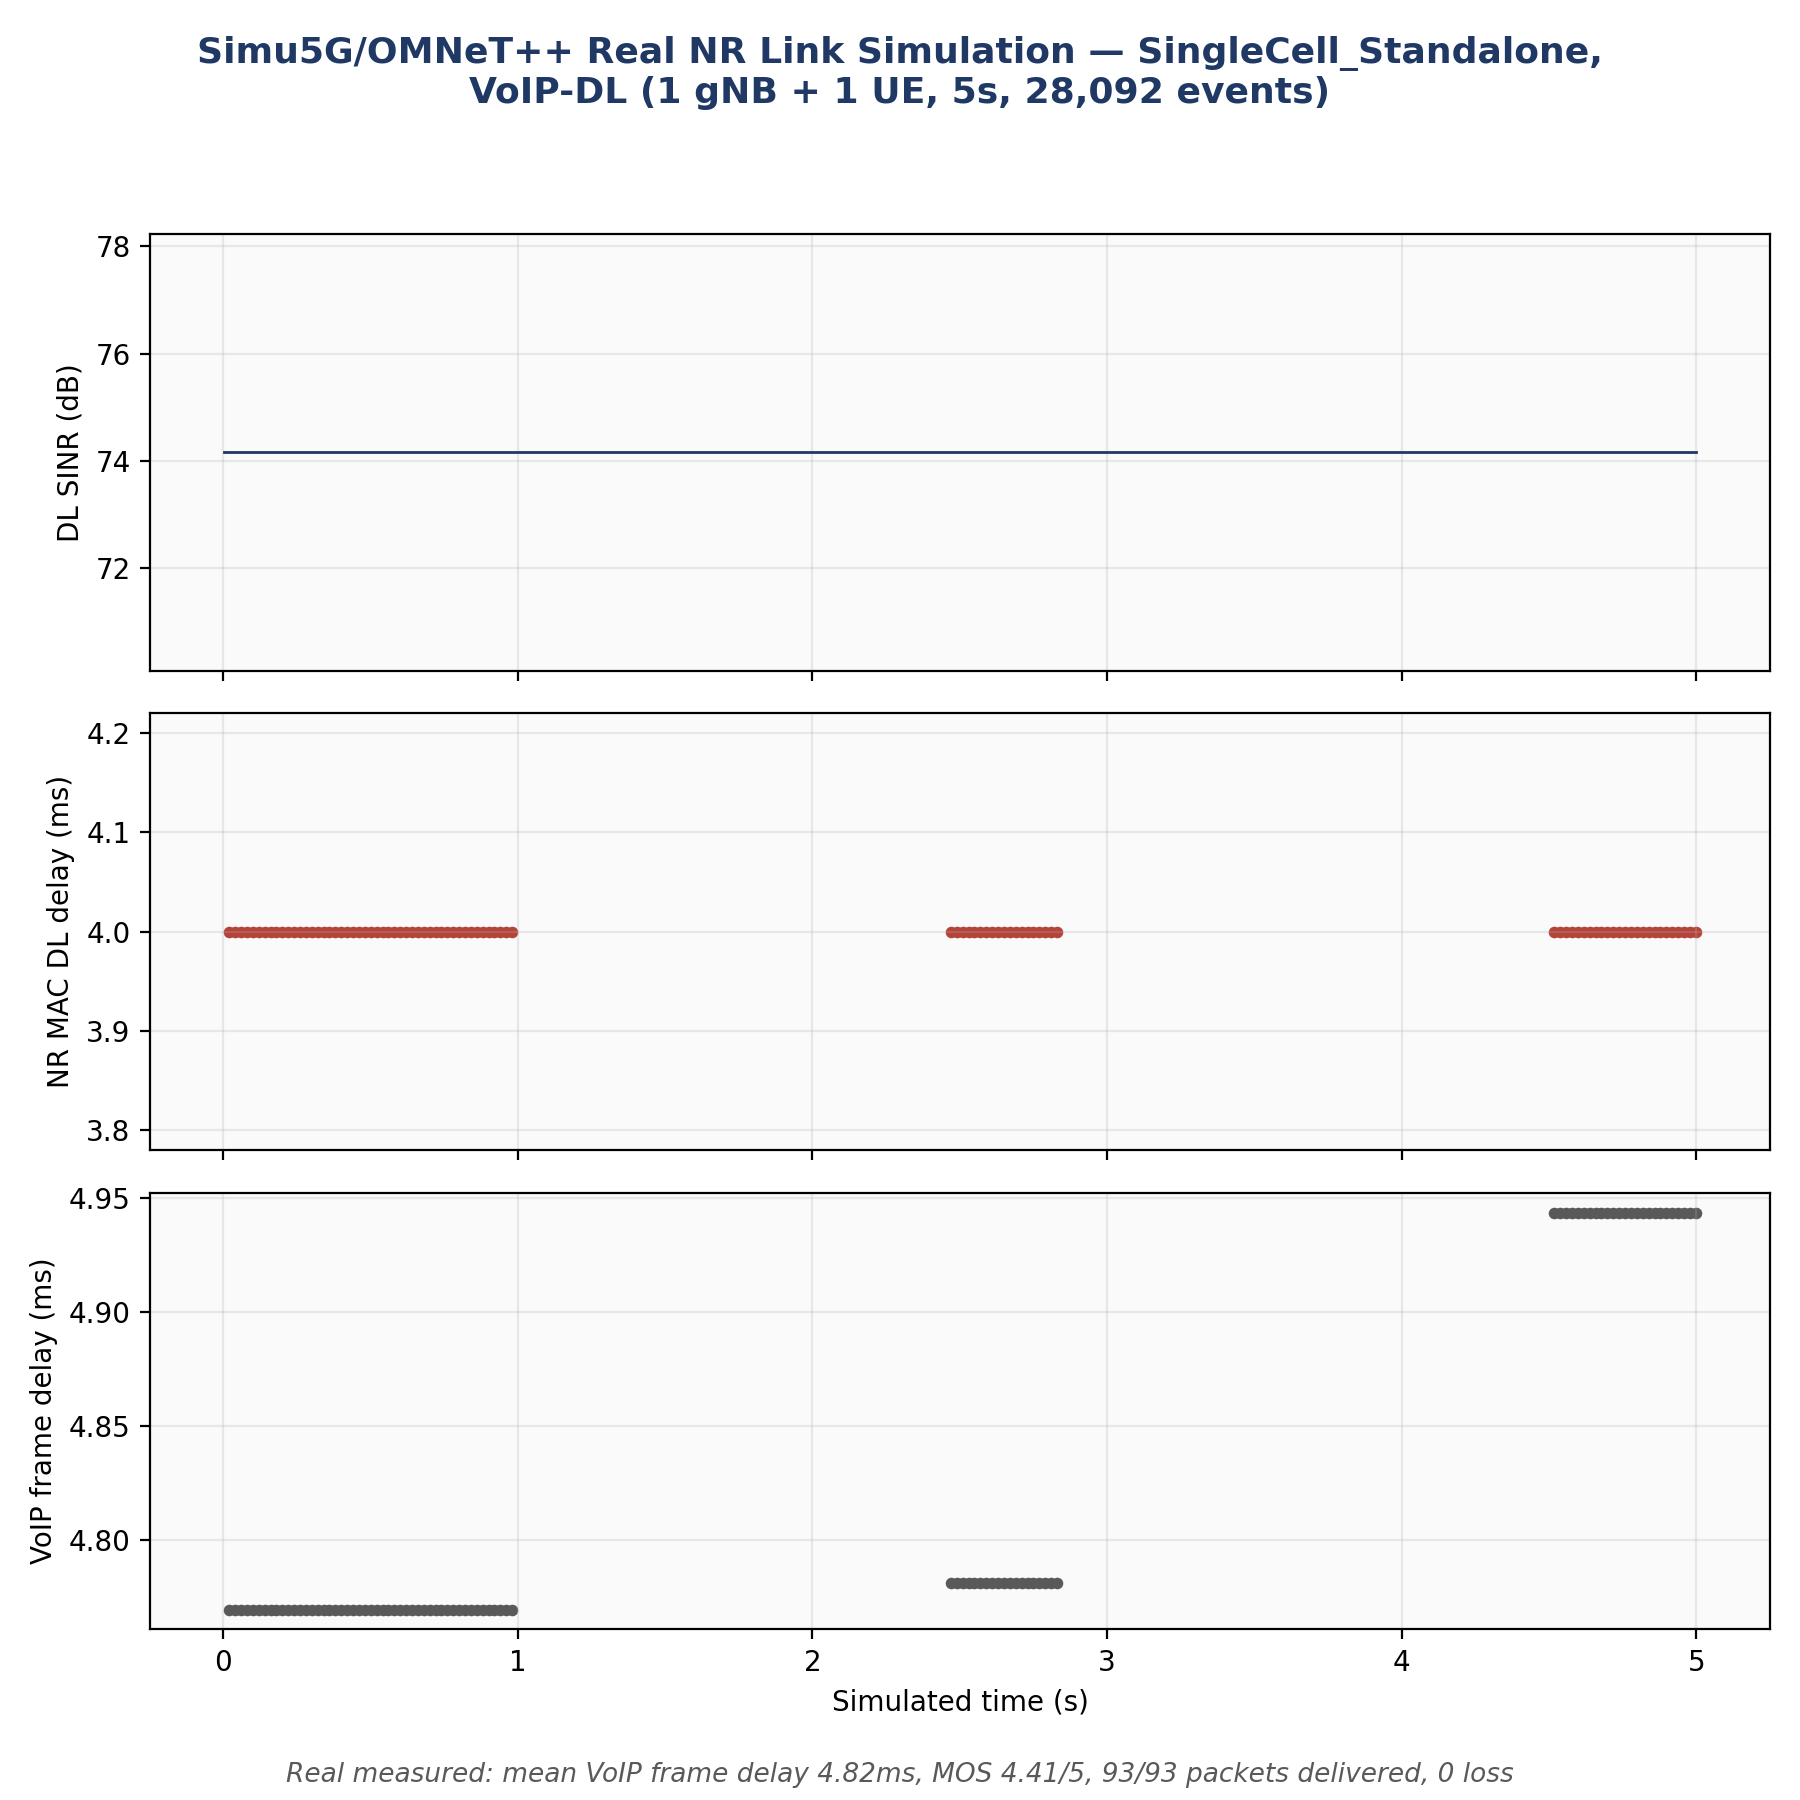
\includegraphics[width=0.75\textwidth,
                     keepaspectratio]{simu5g_ref.png}
    \caption{Reference Simu5G NR run (one gNodeB, one UE, 5 s, downlink VoIP)}
    \label{fig:simu5g}
\end{figure}

\section{Summary}
The unified environment has real traffic and topology from Milan, slice demand, a latency and jitter model calibrated on 6G RAN telemetry, interference from neighbouring cells, and the reward of Equation~(\ref{eq:reward}). It allows forecasting and allocation to be tested together on the same traffic and compared with equal-split, proportional and expert policies, including tuned versions. Its main limit is the surrogate QoS model, which Chapter~\ref{chap.8} compares with a packet-level simulator.
